\documentclass[12pt]{article}%
\usepackage{amsfonts}
\usepackage{amsmath}
\usepackage{amsthm}
\usepackage[a4paper, top=2.5cm, bottom=2.5cm, left=2.2cm, right=2.2cm]%
{geometry}
\usepackage{times}
\usepackage{parskip}
\usepackage{complexity}
\usepackage{graphicx}
\usepackage{physics}
\usepackage{mdframed}
\usepackage{amsmath}
\usepackage{amssymb}
%\newenvironment{proof}[1][Proof]{\textbf{#1.} }{\ \rule{0.5em}{0.5em}}
\DeclareMathOperator{\im}{im}
\theoremstyle{definition}
\newmdtheoremenv{definition}{Definition}
\newmdtheoremenv{theorem}{Theorem}
\newmdtheoremenv{prop}{Proposition}
\setlength{\parskip}{2pt}
\setlength{\parindent}{15pt}

\begin{document}

\title{Product Constructions in Homological Quantum Codes}
\author{Edward Kim}
\date{\today}
\maketitle

\begin{abstract}
In this report, we briefly outline Homological Quantum Codes and a techinique introduced by Tillich-Z\'emor to create new quantum codes using a specific type of graph product operation. This product operation can take two classical linear LDPC codes as input to produce a CSS code with constant encoding rate and distance scaling to a square root of the number of physical qubits. It is defined using $X$-type and $Z$-type stabilizers can be respectively identified through the image of a certain boundary map and its transpose on a family of binary vector spaces. Finally, we touch on a few implications and generalizations of the product construction.
\end{abstract}

\section{Introduction}

\hspace{\parindent}Throughout the semester, we discussed several types of quantum error correction schemes and their modus operandi for correcting quantum errors. A recent research effort begetting a formidable flurry of beautiful, deep theoretical results is motivated by the construction of quantum analogues of Low Density Parity Check (LDPC) codes \cite{breuckmann2021quantum}. Given a family of classical linear codes $\{\mathcal{C}_n\}_{n \in \mathbb{N}}$, the family of codes is said to be \emph{LDPC} if the Hamming weights of the rows and columns of corresponding parity check matrix of the $\mathcal{C}_n$ are bounded by a universal constant in the limit $n \rightarrow \infty$. 
% \parskip

Classical LDPC codes were found to exhibit efficient decoding algorithms based on belief-propagation. Certain families of LDPC Codes saturate the upper bound on channel capacity conferred by Shannon's Theorem \cite{gallager1962low, mackay1999good}. Additionally, classical coding theory contains numerous constructions of \emph{good} LDPC Codes. We say that a family of classical linear codes  $\{\mathcal{C}_n\}_{n \in \mathbb{N}}$ with code parameters $[n,k(n),d(n)]$ is \emph{good} if the encoding rate $k(n) / n $ and the relative distance $d(n) / n$ are non-vanishing in the limit $n \rightarrow \infty$. Equivalently, both $k(n), d(n)$ scale linearly with the number of encoding bits. 

We can easily generalize the two properties above to families of quantum CSS codes. In other words, a CSS code is said to be LDPC if the stablizer weights of the row and columns of the code's parity check matrix in the symplectic representation is bounded by a universal constant in the limit. The extension of the definition of good classical codes to CSS codes also immediate from the definitions. Besides generally exhibiting simpler error syndrome decoding schemes, Gottesman showed that the existence of Quantum LDPC codes implies that the overhead for fault-tolerant quantum computation can reduced to a constant \cite{gottesman2013fault}. 

However, the road to explicitly constructing good quantum LDPC codes has proven to be challenging. For a remarkable amount of time, existing surface codes and their hyperbolic counterparts could not break a square root distance barrier. In other words, existing surface codes had their distances grow asymptotically $O(\sqrt{n})$ despite being LDPC. The landmark Freedman-Meyer-Luo code \cite{freedman2002z2} managed to break this barrier by constructing a particular hyperbolic 3-manifold and reasoning about the code's distance using systolic geometry. This yields a quantum code with parameters $[[n, 2, \Omega(\sqrt{n}\log^{1/4}{n})]]$. Although the distance falls short of scaling linearly, the authors had made a meaningful stride to construct good quantum LDPC codes. To read a comprehensive treatment on the technicalities of this construction, see \cite{fetaya2011homological}.

The significance of designing quantum codes using \emph{homological} invariants began to shine when the $\Omega(\sqrt{n}\log^{1/4}{n})$ barrier was shattered in 2020 through the culmination of several preceding product constructions and probabilistic arguments. The Evra-Kaufman-Z\'emor \cite{evra2020decodable} construction managed to break the ceiling by taking a certain tensor product between a quantum code and a classical code. This produces a quantum code with a distance parameter scaling $O(\sqrt{n} \log{n})$. Although this report cannot touch on the precise details, we will touch upon a preceding product construction that plays an inextricable role in the Evra-Kaufman-Z\'emor code.



%$\left( \begin{matrix} H_Z & 0 \\ 0 & H_X \end{matrix} \right)$
%the encoding rate $k/n$ and the relative distance 


%Yet another perspective for correcting quantum errors derives itselffrom homology theory. 

%\section{Homology}

\section{CSS Codes and Chain Complexes}
\hspace{\parindent}Homological quantum codes and their error-correction properties are bestowed by virtues of \emph{homology theory}. Homology theory roughly studies the construction of invariants of topological spaces. Such an invariant would only be determined by the structure of topological space itself in such a way that two spaces equivalent up to continuous deformations will output the same ``value" of the invariant. We will sketch a cursory treatment of the required background of the product constructions considered in this report. For a formal introduction to Algebraic Topology and Homological Algebra, see \cite{hatcher2005algebraic, weibel1995introduction} respectively.

To be a bit more precise, the algebraic data mentioned above takes its form as a \emph{chain complex}. A chain complex is defined to be a tuple $(C, \partial)$ consisting of a finite family of binary vector spaces and a family of linear maps known as boundary operators. \footnote{The $C_n$ could generally be abelian groups(modules over a ring) with the $\partial$ being group(module) homomorphisms. The complex can also be of infinite length.} The vector spaces $C_n$ are arranged based on a finite sequence of maps:
%
\[ C_{\ell} \xrightarrow{\partial_\ell} C_{\ell - 1} \xrightarrow{\partial_{\ell-1}} C_{\ell - 2} \xrightarrow{\partial_{\ell -2}} \cdots \xrightarrow{\partial_2} C_{1} \xrightarrow{\partial_1} C_0   \]
%
such that $\partial_{i-1}\partial_{i}$ for all $1 \leq i \leq \ell$. Here, by binary vector space, we mean the usual $\mathbb{F}_2$-vector space $\mathbb{F}_2^m$ for some positive integer $m$. The vanishing condition of the boundary operatrs ensure that $\im \partial_{i+1} \subseteq \ker \partial_{i}$. This shows that we can take the quotient vector space $H_n = \ker \partial_{i} / \im \partial_{i+1}$, which we deem as the \emph{$n^{th}$ homology group}. 

A fundamental insight is the formulation of CSS codes as chain complexes through the following identification: Let $\mathcal{C}$ be a CSS code given by the two classical parity check matrices $H_Z, H_X$ responsible for detecting bit-flip and phase-flip errors respectively. Let $C_XC_Z$ denote the subspace of codewords for the two classical codes above. Now consider the below chain complex:
%
\[ C_2 \xrightarrow{H_Z^{T}} C_1 \xrightarrow{H_X} C_0 \]
%
where the spaces $C_0,C_1,C_2$ represent the parity check space for $H_X$, the codeword space $C_Z$, and the parity check space for $H_Z$ respectively. The parity check space refers to the image of the classical parity check matrices $H_Z,H_X$. By setting $\partial_2 = H_Z^{T}$ and $\partial_1 = H_X$, it immediately follows from the commutation relations of $H_Z,H_X$ that $\partial_1\partial_2 = 0$. Hence, the vector spaces and linear maps above form a valid length-three chain complex. The distance $d_Z$ for the code $C_Z$ will be the minimum Hamming weight over all non-trival classes of  $H_1 = \ker \partial_1  / \im \partial_2$. The number of logical qubits will be $k = \dim{H_1}$. To see this, note that we can identify the bit strings in $\ker \partial_1 = \ker H_X$ as those $Z$-errors which are undetectable by $H_X$. Secondly, we see that $\im H_Z^T = \im C_Z$ can be seen as products of $Z$-type stablizers given by $C_Z$. Thus, the coset elements of $H_1$ represent those classes of phase-flip errors that are undetectable by $H_X$  equivalent up to products of $Z$-type stabilizers. These exactly correspond to those elements which act non-trivially on the stabilizer subspace. 

The case for the $X$-distance $d_X$ is similar except now we consider the boundary maps pointing in the opposite direction. We induce this behavior by taking the transpose of both boundary maps $\partial_1^T, \partial_2^T$ as below:

\[ C_2 \xleftarrow{H_Z} C_1 \xleftarrow{H_X^T} C_0  \]

\noindent Note the arrows point in a direction such that the indices of the vector spaces are read in increasing order. This is an example of a \emph{co-chain complex} with the vector space $H^1 = \ker \partial_2 / \im \partial_1$ deemed as the \emph{$1^{st}$ cohomology group}. The cohomological counterparts to the distance and logical qubits are defined similarly.

\noindent Conversely, given such a chain complex of length three, one can always define a CSS code by setting the qubits to be indiced by the basis vectors of $C_1$. Following this suggestion, given the chain complex of binary vector spaces:

\[ C_2 \xrightarrow{\partial_2} C_1 \xrightarrow{\partial_1} C_0 \]

\noindent define $H_Z = \partial_2$ and $H_X = \partial_1^T$. 


% Maybe add surface code example.
\subsection{Toric Code as Homology}
It could be instructive to understand homology through a small toy example: the toric code. Recall that the toric code is defined on an $m \times m$ lattice with the qubits placed along the edges of the lattice. As the qubits are placed along the surface of the torus, the boundaries are periodic. The $X$-type stabilizers act on qubits within neighborhoods of the vertices while the $Z$-type stabilizers act on qubits placed along the boundary edges of the faces. Define the $\mathbb{F}_2$-vector spaces $C_0,C_1,C_2$ where the basis elements are set to be the vertices, edges, and faces of the lattice respectively. The elements of the vector spaces will be formal sums of the basis elements.
%
Define the boundary operators between the vector spaces:
\[ C_2 \xrightarrow{\partial_2} C_1 \xrightarrow{\partial_1} C_0 \]
%
where we first define $\partial_1, \partial_2$ to take edges(faces) of the lattice and map it to a formal sum of the vertices(edges) that comprise the boundary of the edge(face). For example, suppose we had a single face $f$ whose boundary is given by exactly four edges $e_1, e_2, e_3, e_4$. Then $\partial_2(f) = e_1 + e_2 + e_3 + e_4$. Through the same idea, if an edge $e = (v_1,v_2)$ where $v_1,v_2$ are vertices, $\partial_1(e) = v_1 + v_2$. We finish by extending the map linearly to every basis element. Figure \ref{toricfig} demonstrates the behavior of the boundary maps. Notice that the upper-left vertex of the bottom subfigure does not appear in the image of $\partial_1$ since the vertex appears an even number of times in the formal sum.

\begin{figure} \label{toricfig}
 \centering
 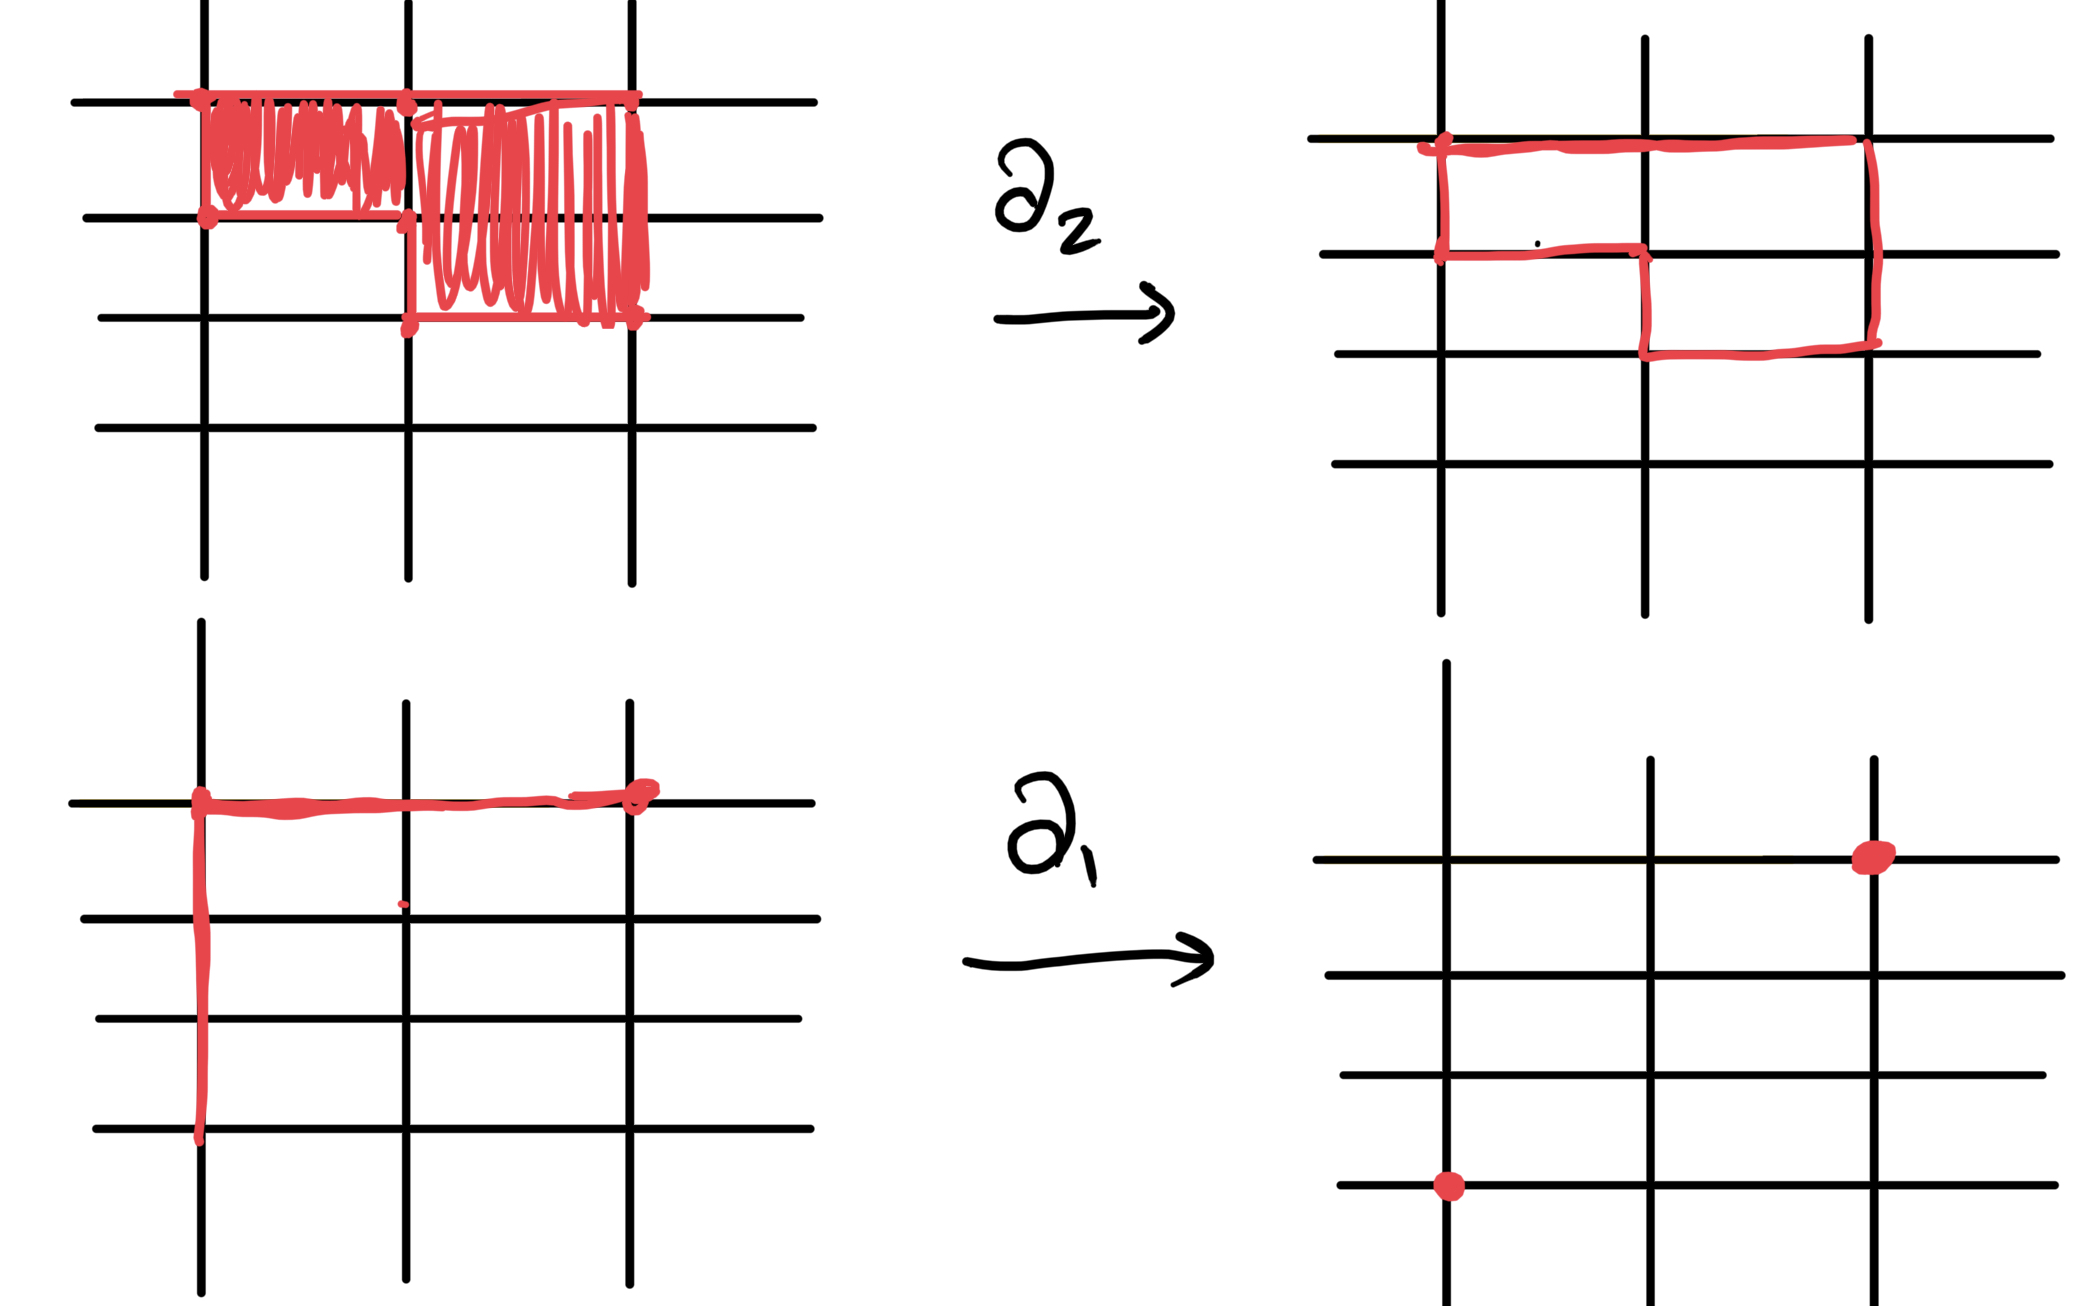
\includegraphics[scale=0.15]{toric}
 \caption{Example of the behavior of the boundary maps of the toric code acting faces and edges. $\partial_1, \partial_2$ depicted bottom and top respectively.}
\end{figure}

A direct calculation shows that $\partial_1\partial_2 = 0$. One can see this by observing that the $\im \partial_2$ necessarily comprises of edges constituting the boundaries of closed regions (union of a subset of lattice faces). By composing the output with $\partial_1$, each vertex appearing as a boundary of an edge will show up an even number of times in formal sum. Thus, the sequence of vector spaces and linear maps above form a valid chain complex. Naturally, we can identify the logical $Z$ operators as elements of non-trivial homology classes contained in $H_1 = \ker \partial_1 / \im \partial_2$. Precisely two of these non-trivial classes represent the logical $Z$-operators acting on the vanilla toric code. 

Finally, we can formalize the machinery for the \emph{dual} lattice in which we consider the faces to be dual vertices and the vertices to be dual faces. This gives the cochain complex:

\[ C_2 \xleftarrow{\partial_2^T} C_1 \xleftarrow{\partial_1^T} C_0  \]

\noindent Note that this is a valid cochain complex since $\partial_2^T\partial_1^T = (\partial_1\partial_2)^T = 0$. Furthermore, the logical $X$-operators are identified as the two non-trivial cohomology classes $H^1 = \ker \partial_2^T / \im \partial_1^T$.  The preceding discussion implies that $Z$-type stabilizers are identified by elements contained in $\im \partial_2$ and the $X$-type stabilizers are identified by $\im \partial_1^T$.



\section{The Tillich-Z\'emor Construction}
One of the earlier efforts investigating a form of product construction was conducted by Tillich-Z\'emor \cite{tillich2013quantum}. The key motivation centers around generalizing the toric code construction by taking the Tanner graphs of two classical binary linear codes and taking a \emph{graph product} of the two graphs. To begin, we first recall a definition:


\vspace{5pt}
\begin{definition}
Let $G_1 = (V_1, E_1)$ and $G_2 = (V_2,E_2)$ denote two undirected graphs. The graph product $G_1 \times G_2$ is defined to be the graph with the following parameters: the vertex set $V$ is designated as $V_1 \times V_2$ and the edge set $E$ contains an edge between $(a,b), (a',b')$ if one of the two criteria are satisfied:

\begin{enumerate}
  \item $a = a'$ and $(b,b') \in E_2$
  \item $b = b'$ and $(a,a') \in E_1$
\end{enumerate}
\end{definition}
\vspace{5pt}

Let $G_1$ and $G_2$ be arbitrary undirected graphs. Consider the output product graph $G_1 \times G_2$. Besides the vertices indiced by tuples in $V_1 \times V_2$, we can try to define faces as cycles of length four arising from two edges $(a,b) \in E_1$ and $(x,y) \in E_2$. A natural attempt at generalizing the toric code could start by defining the $X$-type stablizers to act on incident edges of vertices and $Z$-type stabilizers to act on incident edges of faces. In fact, one can directly verify that the toric code on an $m \times m$ lattice can be casted as a product graph of two cycles of length $m$ stabilized by the generators defined by this scheme. 

To ensure that we can extract a CSS code from a graph product, a more careful construction of the parity check matrices $H_Z, H_X$ must be considered before moving further: Consider a classical binary linear code with some $(n-k) \times n$ parity check matrix $H$. Define  $\mathcal{T}(V,C,E)$ to be a bipartite graph called \emph{Tanner graph}, which has a edge between a variable node $v \in V$ and a check node $c \in C$ if $H_{cv} = 1$. Here, we are essentially indicing the $n-k$ rows of $H$ by check nodes and the $n$ columns by variable nodes.


\vspace{7pt}
\begin{definition}
  Let $G_1 = \mathcal{T}(V_1, C_1, E_1)$ and $G_2 = \mathcal{T}(V_2, C_2, E_2)$. Define   \begin{gather*}
    V := V_1 \times V_2 \cup C_1 \times C_2 \\
    C := V_1 \times C_2 \cup V_2 \times C_1
  \end{gather*}
  Observe that $V \cup C$ gives all nodes in the product graph $G_1 \times G_2$. Additionally, set $G_1 \times_X G_2$ to be the induced bipartite subgraph when restricting $G_1 \times G_2$ to the nodes $V \cup (C_1 \times V_2)$. The induced subgraph $G_1 \times_Z G_2$ to be similar except restricted to the nodes $V \cup (C_2 \times V_1)$. Set $\mathcal{C}(G_1 \times G_2)$ to be the quantum code such that the parity check matrix $H_X$ is described by the Tanner graph $G_1 \times_X G_2$ and $H_Z$ is described by $G_1 \times_Z G_2$. We refer to the corresponding linear codes as $\mathcal{C}_X = \mathcal{C}_X(G_1 \times G_2)$ and $C_Z = \mathcal{C}_Z(G_1 \times G_2)$.
\end{definition}
\vspace{5pt}

\noindent First and foremost, $\mathcal{C}(G_1 \times G_2)$ is actually a CSS code:

\vspace{7pt}
\begin{theorem} \cite{tillich2013quantum}
  Let $G_1,G_2$ be the Tanner graphs defined above. Then $\mathcal{C}_X(G_1 \times G_2)^{\perp} \subset \mathcal{C}_Z(G_1 \times G_2)$. 
\end{theorem}
\vspace{5pt}

\noindent Furthermore, it is possible to cleverly calculate the number of logical qubits for $\mathcal{C}(G_1 \times G_2)$ using a sort of dual of the input Tanner graphs:

\vspace{7pt}
\begin{prop} \cite{tillich2013quantum} \label{logqbit}
  For $i = 1,2$, let $G_i$ be the Tanner graphs for two binary codes $C_i$. If $k_i = \dim{C_i}$ and $k_i^T = \dim{C_i^T}$, then the number of logical qubits encoded by the output CSS code will satisfy
\[k_P = k_1k_2 + k_1^Tk_2^T \]
where $C_i^T$ is the code derived from the \emph{transpose Tanner graph} of $C_i$.
\end{prop}
\vspace{5pt}

\noindent The transpose Tanner graph is simply the original Tanner graph with the variable and check nodes interchanged:

\vspace{7pt}
\begin{definition}
  Given a Tanner graph $G = \mathcal{T}(V, C, E)$, its transpose $G^T$ is given by $G^T = \mathcal{T}(C,V,E)$
\end{definition}
\vspace{5pt}

\noindent Finally, the authors use properties of the hypergraph product of two Tanner graphs and their transposes to find a lower bound on the distance of the output CSS code:

\vspace{7pt}
\begin{theorem} \cite{tillich2013quantum} \label{distance}
For $i = 1,2$, let $d_i$ be the minimum distance of the code described by a Tanner graph $G_i$ and $d_i^T$ be the minimum distance for the code described by the transpose Tanner graph $G_i^T$. Then the minimum distance of the output CSS code $d_P$ will satisfy

\[ d_P \geq \min \{d_1, d_2, d_1^T, d_2^T \} \]
\end{theorem}
\vspace{5pt}

\noindent By invoking Proposition \ref{logqbit} and Theorem \ref{distance} with a classical $[n,k,d]$ 
LDPC code $C$, we arrive at the following result:

\vspace{7pt}
\begin{theorem} \cite{tillich2013quantum} 
  There exists a quantum LDPC code with parameters $[[N, k^2, d]]$ where $N = n^2 + (n-k)^2$.
\end{theorem}
\vspace{5pt}

\noindent This code is constructed by considering \emph{both} input Tanner graphs to be that of the supplied classical LDPC code $C$. Finally, observe that since $d$ scales linearly in $n$, $d \in O(\sqrt{N})$. Evidently, the output CSS code does not break the square root distance barrier.

%\section{Bravyi-Hastings Construction}

\section{Outlook and Discussion}

Since the Tillich-Z\'emor construction, several other improvements and generalizatons have been proposed. A generalization of this construction was considered by Bravyi-Hastings. Their product construction utilized an actual product chain complex to construct CSS codes from two random CSS codes $[[n_1,k_1,d_1]], [[n_2,k_2,d_2]]$ with the same fixed lengths $n_1 = n_2 = \sqrt{n}$ and the same constant encoding rate $k_b = \rho\cdot n_b$ for $\rho > 0, b=1,2$. Addtionally, these random CSS codes are \emph{good} codes in the sense discussed in the first section in this report. The authors showed that the product CSS code is also good with high probability but the stabilizer weights found in the rows and columns of the parity matrix is only upper-bounded by $2\sqrt{n}$:

\vspace{7pt}
\begin{theorem} \cite{bravyi2014homological}
  There exists a family of good CSS codes with stabilizer weight $\leq 2\sqrt{n}$.
\end{theorem} 
\vspace{5pt}

\noindent A major difference between the Tillich-Z\'emor and the Bravyi-Hasting constructions is that the hypergraph product yields a CSS code which is LDPC but not good. On the other hand, the Bravyi-Hastings method produces good CSS codes which may not be LDPC. Another advantage of the Bravyi-Hastings method lies in their use of a product chain complex, which may be defined for any pair of arbitrary chain complexes:

\vspace{7pt}
\begin{definition}
  Suppose we have two chain complexes $(C, \partial), (C', \partial')$ of say binary vector spaces. We define the tensor product of these two complexes by the tuple $(C \otimes C',\partial'')$ where $(C \otimes C')_n = C_n \otimes C'_n.$ and $\partial'' = \partial \otimes I + I \otimes \partial'$.
\end{definition}
\vspace{5pt}
%
\noindent Indeed, $\partial''_{i-1}\partial''_{i} = \partial^2 \otimes I + 2(\partial \otimes \partial'') + I \otimes( \partial'')^2 = 0$ since $\partial^2 = \partial'^2 = 0$ and we are working in a binary vector space. This demonstates that $(C \otimes C',\partial'')$ is a chain complex. This product operation turns out to be a natural generalization of the hypergraph product \cite{freedman2013quantum}. \newline

\noindent It is worth nothing a few other generalized and more recent product constructions:

\begin{enumerate}
  \item In the introduction, we mentioned that Evra-Kaufman-Z\'emor have generalized a \emph{distance balancing} operation to break the Freedman-Meyer-Luo distance record. Using high-dimensional expanders on Ramanujan complexes, they roughly proved that specific tensor product between a classical $[m, q, d]$ code with $\ell$ parity checks and a $[[n, k ,d_X, d_Z]]$ quantum CSS code with $\ell_X$ $X$-type stablizers creates a $[[nm + \ell_X\ell, kq, d_X, d_Zd]]$ quantum code. Note the increased $Z$-distance $d_Zd$ relative to the $X$-distance $d_X$. By exploiting distance balancing to a quantum code first derived from Ramanujan complexes, the authors remarkably were able to exhibit a code with distance $d \in O(\sqrt{n} \sqrt{\log{n}})$.
  \item Several months later, Kaufman-Tessler \cite{kaufman2021new} broke the distance barrier once more by taking iterated tensor products of Ramanujan complexes. Their code produced a distance parameter of $d \in O(\sqrt{n} \log^m{n})$.
  \item Panteleev-Kalachev introduced a \emph{generalized hypergraph product (GHC)} \cite{panteleev2021degenerate} with which they remarkably showed how to beat the previous distance record by Hastings-Haah-O'donnell's Fiber Bundle Code \cite{hastings2021fiber}. The original GHC method is tailored to specific codes considered by Sipser-Spielman expander codes \cite{sipser1996expander}, yielding families of quantum LDPC codes with logical bits $\Theta(n^\alpha \log{n})$ and distance $\Theta(n^{1 - \alpha/2}\log{n})$ for any $0 \leq \alpha < 1$. Observe the tradeoff between the encoding rate and the distance of the lifted code. Due to this, the code falls slightly short of being both a good quantum code and a quantum LDPC code.
  \item Breuckmann-Eberhardt introduced \emph{balanced product codes} \cite{breuckmann2021balanced} around the same time period as the GHC construction was developed. Like the GHC construction, the balanced product construction roughly depends on a reducton of symmetry of the tensor product. Here, the product takes two classical codesrespecting some common symmetry expressed as a group. By taking a balanced product between the Sipser-Spielman expander codes and repetition codes with cyclic symmetry, they are able to construct \emph{non-random} families of quantum codes with parameters $[[n, \Omega(n^{4/5}), \Omega(n^{3/5})]]$. Compare this with the approaches mentioned above whose arguments on the bounds of the code parameters only hold with high probability when taking products of random CSS codes or random classical linear codes. 
\end{enumerate}



    %Each product construction considers a intriguing perspective on bolstering or attenutating the code parameters. It is worth noting that all these product constructions have been analyzed and designed over the past two years. This sudden uptick in research activity is further kindled by the drive to construct \emph{good} quantum LDPC codes. 

        In conclusion, product constructions in Homological Quantum Codes are a beautiful, propituous mixture of Algebraic Topology, Homological Algebra, and Quantum Error Correction. The existence of good quantum LDPC codes also have wide-reaching implications in other fields of study. For example, the construction of good quantum LDPC codes could shed more light on the Quantum PCP conjecture and the NTLS conjecture \cite{aharonov2013guest, freedman2013quantum}. It is also interesting to see what other unexplored tools and ideas from Algebraic Topology and Differential Geometry could bestow interesting results in quantum LDPC codes.



%Twistings
%Lifted Products
%generalized hypergraph.
%hastings manifold


\bibliographystyle{abbrv}
\bibliography{biblio}

\end{document}
